\documentclass{article}\usepackage[]{graphicx}\usepackage[]{color}
%% maxwidth is the original width if it is less than linewidth
%% otherwise use linewidth (to make sure the graphics do not exceed the margin)
\makeatletter
\def\maxwidth{ %
  \ifdim\Gin@nat@width>\linewidth
    \linewidth
  \else
    \Gin@nat@width
  \fi
}
\makeatother

\definecolor{fgcolor}{rgb}{0.345, 0.345, 0.345}
\newcommand{\hlnum}[1]{\textcolor[rgb]{0.686,0.059,0.569}{#1}}%
\newcommand{\hlstr}[1]{\textcolor[rgb]{0.192,0.494,0.8}{#1}}%
\newcommand{\hlcom}[1]{\textcolor[rgb]{0.678,0.584,0.686}{\textit{#1}}}%
\newcommand{\hlopt}[1]{\textcolor[rgb]{0,0,0}{#1}}%
\newcommand{\hlstd}[1]{\textcolor[rgb]{0.345,0.345,0.345}{#1}}%
\newcommand{\hlkwa}[1]{\textcolor[rgb]{0.161,0.373,0.58}{\textbf{#1}}}%
\newcommand{\hlkwb}[1]{\textcolor[rgb]{0.69,0.353,0.396}{#1}}%
\newcommand{\hlkwc}[1]{\textcolor[rgb]{0.333,0.667,0.333}{#1}}%
\newcommand{\hlkwd}[1]{\textcolor[rgb]{0.737,0.353,0.396}{\textbf{#1}}}%

\usepackage{framed}
\makeatletter
\newenvironment{kframe}{%
 \def\at@end@of@kframe{}%
 \ifinner\ifhmode%
  \def\at@end@of@kframe{\end{minipage}}%
  \begin{minipage}{\columnwidth}%
 \fi\fi%
 \def\FrameCommand##1{\hskip\@totalleftmargin \hskip-\fboxsep
 \colorbox{shadecolor}{##1}\hskip-\fboxsep
     % There is no \\@totalrightmargin, so:
     \hskip-\linewidth \hskip-\@totalleftmargin \hskip\columnwidth}%
 \MakeFramed {\advance\hsize-\width
   \@totalleftmargin\z@ \linewidth\hsize
   \@setminipage}}%
 {\par\unskip\endMakeFramed%
 \at@end@of@kframe}
\makeatother

\definecolor{shadecolor}{rgb}{.97, .97, .97}
\definecolor{messagecolor}{rgb}{0, 0, 0}
\definecolor{warningcolor}{rgb}{1, 0, 1}
\definecolor{errorcolor}{rgb}{1, 0, 0}
\newenvironment{knitrout}{}{} % an empty environment to be redefined in TeX

\usepackage{alltt}

\title{Problem Set 1}
\author{Tony Lashley}
\date{April 6, 2015}

\usepackage{natbib}
\usepackage{graphicx}
\graphicspath{{/Users/Tony/Pictures/}}
\IfFileExists{upquote.sty}{\usepackage{upquote}}{}
\begin{document}
\maketitle

\section{Getting Started with R}
\subsection{Print inline “hello world”}

\begin{knitrout}
\definecolor{shadecolor}{rgb}{0.969, 0.969, 0.969}\color{fgcolor}\begin{kframe}
\begin{alltt}
\hlkwd{print}\hlstd{(}\hlstr{'hello world'}\hlstd{,} \hlkwc{quote}\hlstd{=}\hlnum{FALSE}\hlstd{)}
\end{alltt}
\begin{verbatim}
## [1] hello world
\end{verbatim}
\end{kframe}
\end{knitrout}

\subsection{Create a vector y}
\begin{knitrout}
\definecolor{shadecolor}{rgb}{0.969, 0.969, 0.969}\color{fgcolor}\begin{kframe}
\begin{alltt}
\hlstd{y} \hlkwb{<-} \hlkwd{c}\hlstd{(}\hlnum{100}\hlstd{,}\hlnum{200}\hlstd{,}\hlnum{300}\hlstd{,}\hlnum{400}\hlstd{,}\hlnum{500}\hlstd{)}
\hlkwd{print}\hlstd{(y)}
\end{alltt}
\begin{verbatim}
## [1] 100 200 300 400 500
\end{verbatim}
\end{kframe}
\end{knitrout}

\subsection{Create normal matrix x with mean 100 and variance 10}
\begin{knitrout}
\definecolor{shadecolor}{rgb}{0.969, 0.969, 0.969}\color{fgcolor}\begin{kframe}
\begin{alltt}
\hlkwd{set.seed}\hlstd{(}\hlnum{20866}\hlstd{)}
\hlstd{x} \hlkwb{<-} \hlkwd{matrix}\hlstd{(}\hlkwd{rnorm}\hlstd{(}\hlnum{5}\hlopt{*}\hlnum{5}\hlstd{,} \hlkwc{mean} \hlstd{=} \hlnum{100}\hlstd{,} \hlkwc{sd} \hlstd{=} \hlkwd{sqrt}\hlstd{(}\hlnum{10}\hlstd{)),} \hlnum{5}\hlstd{,} \hlnum{5}\hlstd{)}
\hlkwd{print}\hlstd{(x)}
\end{alltt}
\begin{verbatim}
##           [,1]      [,2]      [,3]      [,4]      [,5]
## [1,]  97.35727 103.97484 103.36721 105.37185 103.32458
## [2,]  99.13215  95.49546 100.97945  99.76002 102.88952
## [3,]  97.39839  96.15575  99.58361  97.97385 100.40162
## [4,]  99.85983  98.78686 103.37817 102.47731 103.00107
## [5,] 102.50208  99.03253  97.78627  96.32905  99.71611
\end{verbatim}
\end{kframe}
\end{knitrout}

\subsection{Calculate and display (X prime X) inverse}
\begin{knitrout}
\definecolor{shadecolor}{rgb}{0.969, 0.969, 0.969}\color{fgcolor}\begin{kframe}
\begin{alltt}
\hlstd{xprime} \hlkwb{<-} \hlkwd{t}\hlstd{(x)}
\hlstd{xAndPrimeMultiplied} \hlkwb{<-} \hlstd{xprime} \hlopt \hlstd{x}
\hlstd{xSolution} \hlkwb{<-} \hlkwd{solve}\hlstd{(xAndPrimeMultiplied)}
\hlkwd{print}\hlstd{(xSolution)}
\end{alltt}
\begin{verbatim}
##            [,1]       [,2]       [,3]       [,4]       [,5]
## [1,]  0.2771095 -0.2351883 -0.3306888  0.5802069 -0.2859665
## [2,] -0.2351883  0.2402567  0.3475531 -0.5498854  0.1936152
## [3,] -0.3306888  0.3475531  1.2137628 -1.0664347 -0.1672556
## [4,]  0.5802069 -0.5498854 -1.0664347  1.4540417 -0.4079109
## [5,] -0.2859665  0.1936152 -0.1672556 -0.4079109  0.6589055
\end{verbatim}
\begin{alltt}
\hlstd{crossProductX} \hlkwb{<-} \hlkwd{crossprod}\hlstd{(x)}
\hlstd{xSolution2} \hlkwb{<-} \hlkwd{solve}\hlstd{(crossProductX)}
\hlkwd{print}\hlstd{(xSolution2)}
\end{alltt}
\begin{verbatim}
##            [,1]       [,2]       [,3]       [,4]       [,5]
## [1,]  0.2771095 -0.2351883 -0.3306888  0.5802069 -0.2859665
## [2,] -0.2351883  0.2402567  0.3475531 -0.5498854  0.1936152
## [3,] -0.3306888  0.3475531  1.2137628 -1.0664347 -0.1672556
## [4,]  0.5802069 -0.5498854 -1.0664347  1.4540417 -0.4079109
## [5,] -0.2859665  0.1936152 -0.1672556 -0.4079109  0.6589055
\end{verbatim}
\end{kframe}
\end{knitrout}

\subsection{Calculate sum of entries in y}
\begin{knitrout}
\definecolor{shadecolor}{rgb}{0.969, 0.969, 0.969}\color{fgcolor}\begin{kframe}
\begin{alltt}
\hlstd{sumYEntries} \hlkwb{<-} \hlkwd{sum}\hlstd{(y)}
\hlkwd{print}\hlstd{(sumYEntries)}
\end{alltt}
\begin{verbatim}
## [1] 1500
\end{verbatim}
\end{kframe}
\end{knitrout}

\subsection{Calculate row sums of X}
\begin{knitrout}
\definecolor{shadecolor}{rgb}{0.969, 0.969, 0.969}\color{fgcolor}\begin{kframe}
\begin{alltt}
\hlstd{xRowSums} \hlkwb{<-} \hlkwd{rowSums}\hlstd{(x)}
\hlkwd{print}\hlstd{(xRowSums)}
\end{alltt}
\begin{verbatim}
## [1] 513.3957 498.2566 491.5132 507.5032 495.3660
\end{verbatim}
\end{kframe}
\end{knitrout}

\subsection{Return maximum value in X}
\begin{knitrout}
\definecolor{shadecolor}{rgb}{0.969, 0.969, 0.969}\color{fgcolor}\begin{kframe}
\begin{alltt}
\hlstd{xMax} \hlkwb{<-} \hlkwd{max}\hlstd{(x)}
\hlkwd{print}\hlstd{(xMax)}
\end{alltt}
\begin{verbatim}
## [1] 105.3718
\end{verbatim}
\end{kframe}
\end{knitrout}

\subsection{Replace third row of X with zeroes}
\begin{knitrout}
\definecolor{shadecolor}{rgb}{0.969, 0.969, 0.969}\color{fgcolor}\begin{kframe}
\begin{alltt}
\hlstd{newMatrix} \hlkwb{<-} \hlstd{x}
\hlstd{z} \hlkwb{<-} \hlkwd{c}\hlstd{(}\hlnum{0}\hlstd{,} \hlnum{0}\hlstd{,} \hlnum{0}\hlstd{,} \hlnum{0}\hlstd{,} \hlnum{0}\hlstd{)}
\hlstd{newMatrix[}\hlnum{3}\hlstd{, ]}\hlkwb{<-} \hlstd{z}
\hlkwd{print}\hlstd{(newMatrix)}
\end{alltt}
\begin{verbatim}
##           [,1]      [,2]      [,3]      [,4]      [,5]
## [1,]  97.35727 103.97484 103.36721 105.37185 103.32458
## [2,]  99.13215  95.49546 100.97945  99.76002 102.88952
## [3,]   0.00000   0.00000   0.00000   0.00000   0.00000
## [4,]  99.85983  98.78686 103.37817 102.47731 103.00107
## [5,] 102.50208  99.03253  97.78627  96.32905  99.71611
\end{verbatim}
\end{kframe}
\end{knitrout}

\section{Function and Loops in R}
\subsection{Use for loop to print all numbers between 1 and 100 which are not multiples of 3 or 4}
\begin{knitrout}
\definecolor{shadecolor}{rgb}{0.969, 0.969, 0.969}\color{fgcolor}\begin{kframe}
\begin{alltt}
\hlkwa{for} \hlstd{(n} \hlkwa{in} \hlnum{1}\hlopt{:}\hlnum{100}\hlstd{)}
  \hlkwa{if} \hlstd{(((n}\hlopt\hlnum{3}\hlstd{)} \hlopt{!=} \hlnum{0}\hlstd{)} \hlopt{&} \hlstd{((n}\hlopt\hlnum{4}\hlstd{)} \hlopt{!=} \hlnum{0}\hlstd{))\{}
    \hlkwd{print}\hlstd{(n)}
  \hlstd{\}}
\end{alltt}
\begin{verbatim}
## [1] 1
## [1] 2
## [1] 5
## [1] 7
## [1] 10
## [1] 11
## [1] 13
## [1] 14
## [1] 17
## [1] 19
## [1] 22
## [1] 23
## [1] 25
## [1] 26
## [1] 29
## [1] 31
## [1] 34
## [1] 35
## [1] 37
## [1] 38
## [1] 41
## [1] 43
## [1] 46
## [1] 47
## [1] 49
## [1] 50
## [1] 53
## [1] 55
## [1] 58
## [1] 59
## [1] 61
## [1] 62
## [1] 65
## [1] 67
## [1] 70
## [1] 71
## [1] 73
## [1] 74
## [1] 77
## [1] 79
## [1] 82
## [1] 83
## [1] 85
## [1] 86
## [1] 89
## [1] 91
## [1] 94
## [1] 95
## [1] 97
## [1] 98
\end{verbatim}
\end{kframe}
\end{knitrout}

\subsection{Write function for fibonacci numbers less than input}
\begin{knitrout}
\definecolor{shadecolor}{rgb}{0.969, 0.969, 0.969}\color{fgcolor}\begin{kframe}
\begin{alltt}
\hlstd{fibfunction} \hlkwb{<-} \hlkwa{function}\hlstd{(}\hlkwc{x}\hlstd{)\{}

  \hlstd{Fib1} \hlkwb{<-} \hlnum{1}
  \hlstd{Fib2} \hlkwb{<-} \hlnum{1}
  \hlstd{Fibonacci} \hlkwb{<-} \hlstd{Fib1}

    \hlkwa{while} \hlstd{(Fib2} \hlopt{<} \hlstd{x)\{}
      \hlstd{Fibonacci} \hlkwb{<-} \hlkwd{c}\hlstd{(Fibonacci, Fib2)}
      \hlstd{oldFib2} \hlkwb{<-} \hlstd{Fib2}
      \hlstd{Fib2} \hlkwb{<-} \hlstd{Fib1} \hlopt{+} \hlstd{Fib2}
      \hlstd{Fib1} \hlkwb{<-} \hlstd{oldFib2}
    \hlstd{\}}

  \hlkwd{print}\hlstd{(Fibonacci)}
\hlstd{\}}

\hlkwd{fibfunction}\hlstd{(}\hlnum{1000}\hlstd{)}
\end{alltt}
\begin{verbatim}
##  [1]   1   1   2   3   5   8  13  21  34  55  89 144 233 377 610 987
\end{verbatim}
\end{kframe}
\end{knitrout}

\section{Basic Regression in R}
\subsection{Calculate the correlation between X and Y}
\begin{knitrout}
\definecolor{shadecolor}{rgb}{0.969, 0.969, 0.969}\color{fgcolor}\begin{kframe}
\begin{alltt}
\hlkwd{rm}\hlstd{(}\hlkwc{list}\hlstd{=}\hlkwd{ls}\hlstd{())}
\hlkwd{set.seed}\hlstd{(}\hlnum{21410}\hlstd{)}

\hlstd{n} \hlkwb{<-} \hlnum{200}
\hlstd{X} \hlkwb{<-} \hlkwd{rnorm}\hlstd{(n,}\hlnum{20}\hlstd{,}\hlnum{10}\hlstd{)}
\hlstd{eps} \hlkwb{<-} \hlkwd{rnorm}\hlstd{(n,}\hlnum{0}\hlstd{,}\hlnum{4}\hlstd{)}
\hlstd{beta} \hlkwb{<-} \hlnum{3.1}
\hlstd{const} \hlkwb{<-} \hlnum{2}
\hlstd{Y} \hlkwb{<-} \hlstd{const} \hlopt{+} \hlstd{(X} \hlopt{*} \hlstd{beta)} \hlopt{+} \hlstd{eps}
\hlstd{correlation} \hlkwb{<-} \hlkwd{cor}\hlstd{(X,Y)}
\hlkwd{print}\hlstd{(correlation)}
\end{alltt}
\begin{verbatim}
## [1] 0.9909514
\end{verbatim}
\end{kframe}
\end{knitrout}

\subsection{Plot the Y values for each individual (Y on the y-axis, 1-200 on the x-axis)}
\begin{knitrout}
\definecolor{shadecolor}{rgb}{0.969, 0.969, 0.969}\color{fgcolor}\begin{kframe}
\begin{alltt}
\hlkwd{plot}\hlstd{(Y)}
\end{alltt}
\end{kframe}
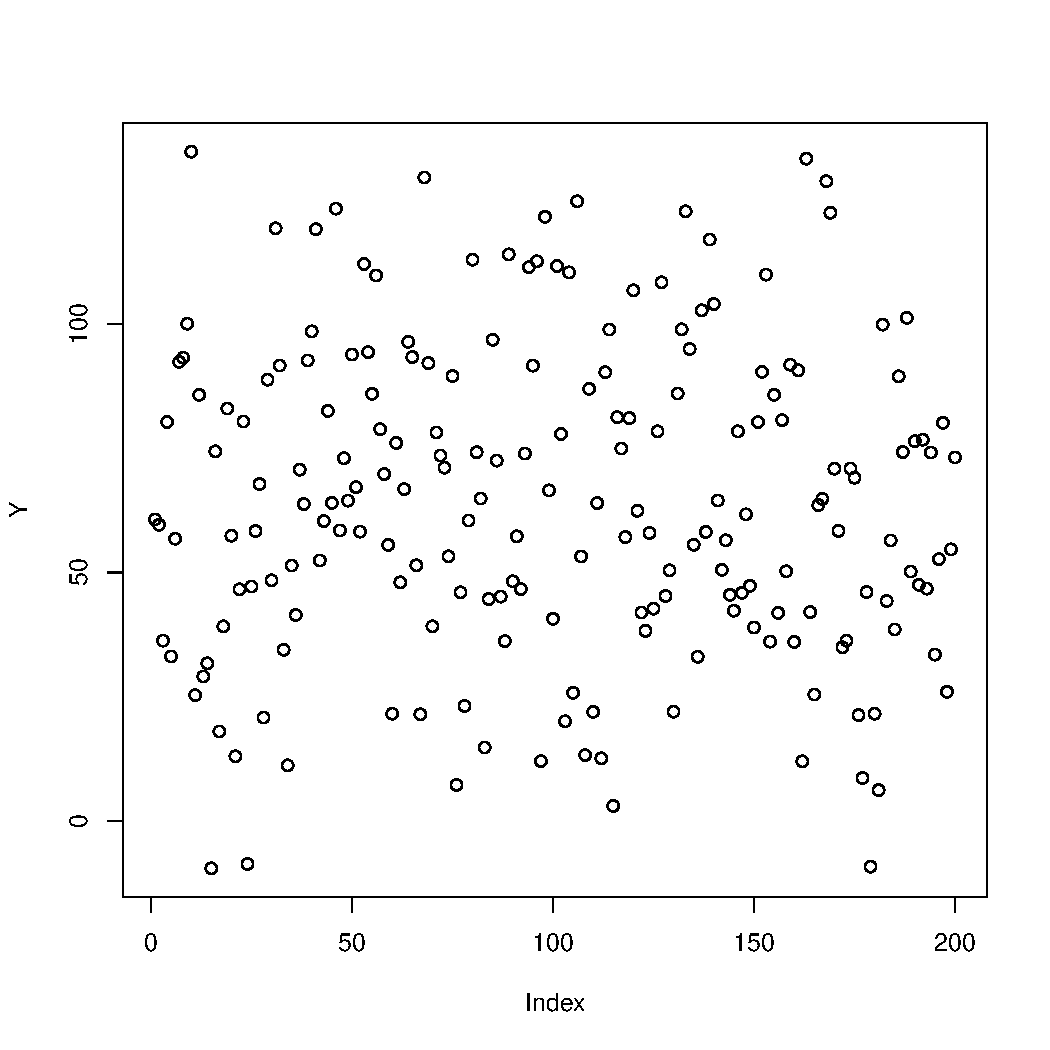
\includegraphics[width=\maxwidth]{figure/unnamed-chunk-12-1} 

\end{knitrout}

\subsection{Plot a histogram of Y}
\begin{knitrout}
\definecolor{shadecolor}{rgb}{0.969, 0.969, 0.969}\color{fgcolor}\begin{kframe}
\begin{alltt}
\hlkwd{hist}\hlstd{(Y)}
\end{alltt}
\end{kframe}
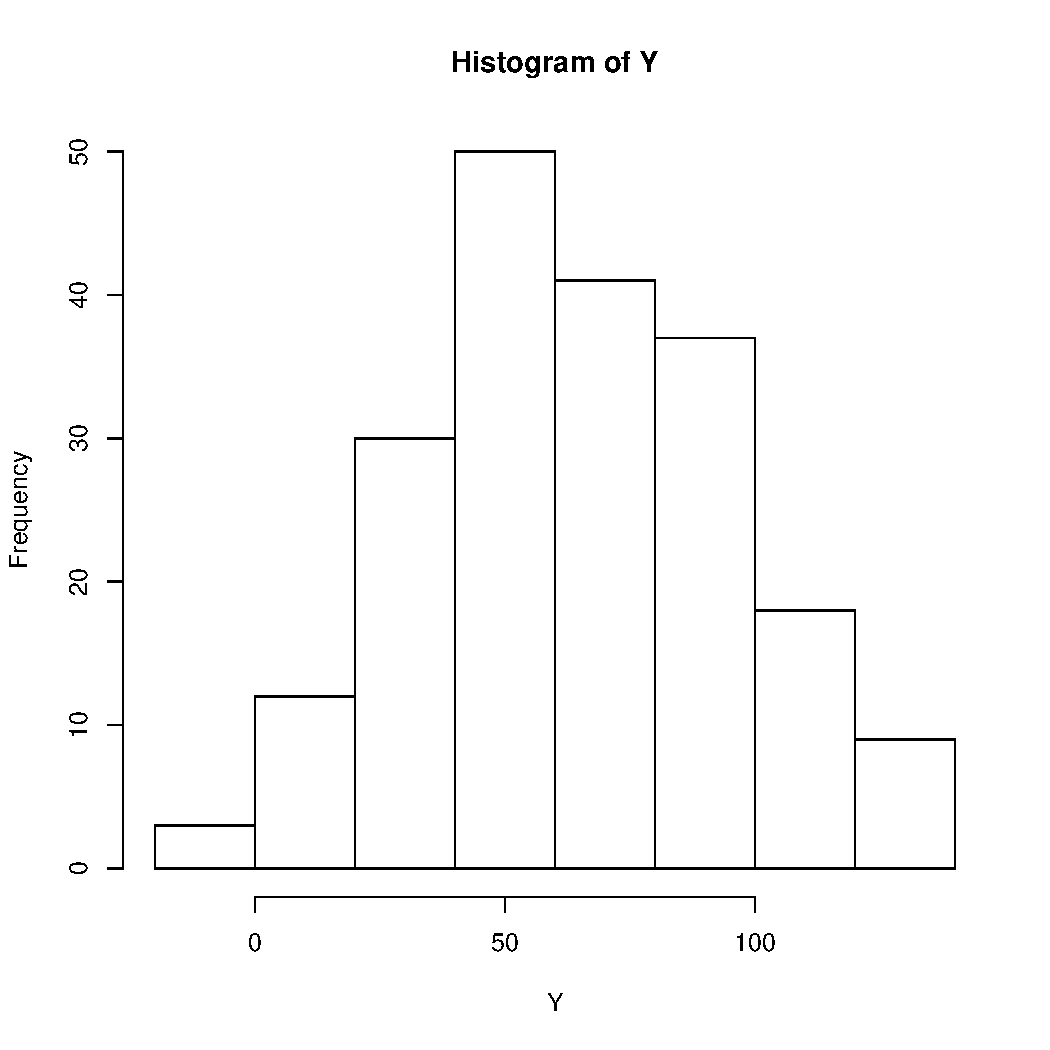
\includegraphics[width=\maxwidth]{figure/unnamed-chunk-13-1} 

\end{knitrout}

\subsection{Plot a histogram of Y using the packages ggplot2 or ggvis}
\begin{knitrout}
\definecolor{shadecolor}{rgb}{0.969, 0.969, 0.969}\color{fgcolor}\begin{kframe}
\begin{alltt}
\hlkwd{library}\hlstd{(ggplot2)}
\hlkwd{qplot}\hlstd{(Y,} \hlkwc{geom}\hlstd{=}\hlstr{"histogram"}\hlstd{)}
\end{alltt}


{\ttfamily\noindent\itshape\color{messagecolor}{\#\# stat\_bin: binwidth defaulted to range/30. Use 'binwidth = x' to adjust this.}}\end{kframe}
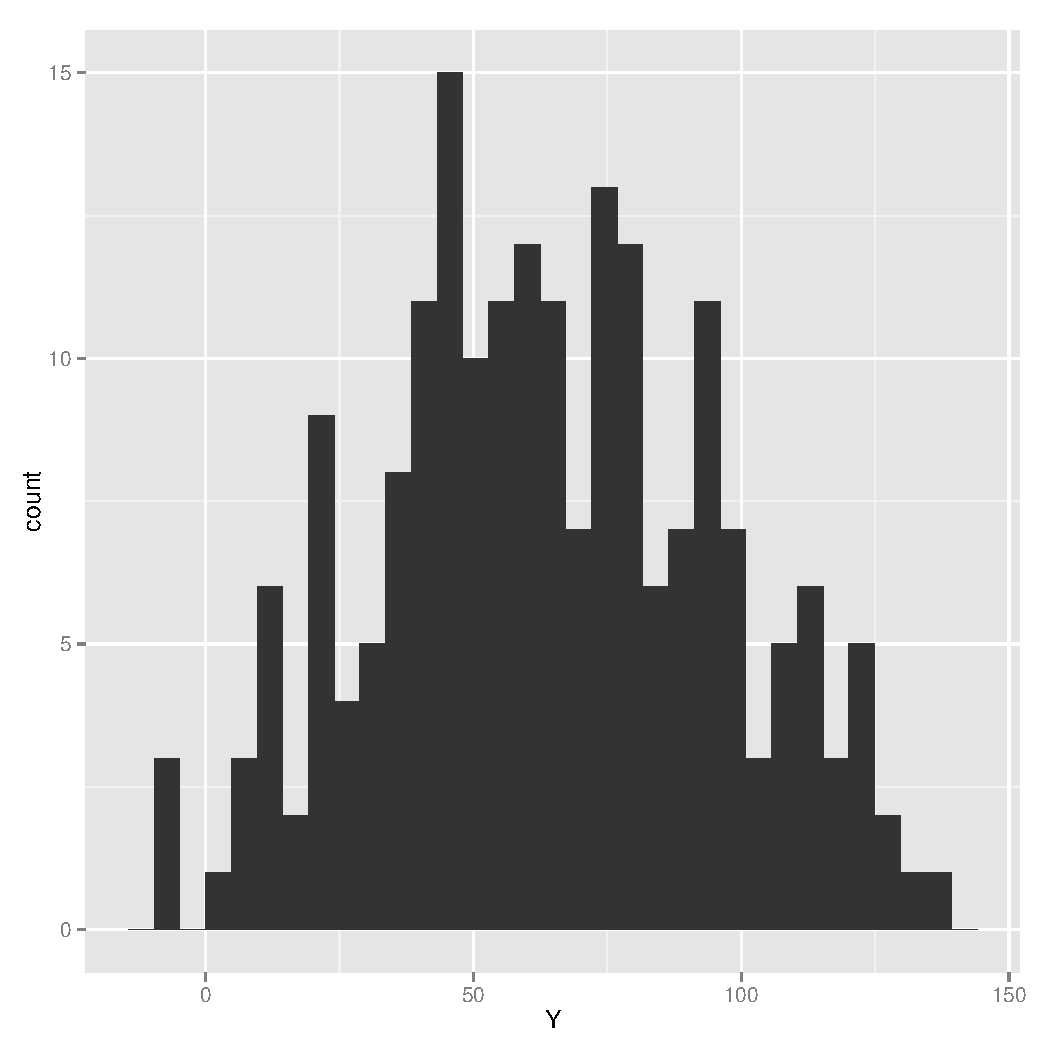
\includegraphics[width=\maxwidth]{figure/unnamed-chunk-14-1} 

\end{knitrout}
\subsection{Use your simulated data to run the regression of Y on X using the lm() command}
\begin{knitrout}
\definecolor{shadecolor}{rgb}{0.969, 0.969, 0.969}\color{fgcolor}\begin{kframe}
\begin{alltt}
\hlstd{fit} \hlkwb{<-} \hlkwd{lm}\hlstd{(Y} \hlopt{~} \hlstd{X)}
\hlstd{fit}
\end{alltt}
\begin{verbatim}
## 
## Call:
## lm(formula = Y ~ X)
## 
## Coefficients:
## (Intercept)            X  
##       1.707        3.100
\end{verbatim}
\end{kframe}
\end{knitrout}

\subsection{Make a latex table of the regression results using xtable() or stargazer()}
\begin{knitrout}
\definecolor{shadecolor}{rgb}{0.969, 0.969, 0.969}\color{fgcolor}\begin{kframe}
\begin{alltt}
\hlkwd{library}\hlstd{(xtable)}
\hlkwd{xtable}\hlstd{(fit)}
\end{alltt}
\begin{verbatim}
## % latex table generated in R 3.1.3 by xtable 1.7-4 package
## % Wed Apr  8 16:03:16 2015
## \begin{table}[ht]
## \centering
## \begin{tabular}{rrrrr}
##   \hline
##  & Estimate & Std. Error & t value & Pr($>$$|$t$|$) \\ 
##   \hline
## (Intercept) & 1.7073 & 0.6719 & 2.54 & 0.0118 \\ 
##   X & 3.1004 & 0.0298 & 103.89 & 0.0000 \\ 
##    \hline
## \end{tabular}
## \end{table}
\end{verbatim}
\end{kframe}
\end{knitrout}

\begin{table}[ht]
\centering
\begin{tabular}{rrrrr}
   \hline
  & Estimate & Std. Error & t value & Pr($>$$|$t$|$) \\
   \hline
 (Intercept) & 1.7073 & 0.6719 & 2.54 & 0.0118 \\
   X & 3.1004 & 0.0298 & 103.89 & 0.0000 \\
    \hline
 \end{tabular}
 \end{table}

\section{Getting Started with Latex}
\subsection{Insert an image off the internet, preferbly a kitten}

\includegraphics{kittycat}

\subsection{Display matrix x and vector y above in Latex}
\begin{knitrout}
\definecolor{shadecolor}{rgb}{0.969, 0.969, 0.969}\color{fgcolor}\begin{kframe}
\begin{alltt}
\hlkwd{options}\hlstd{(}\hlkwc{digits} \hlstd{=} \hlnum{0}\hlstd{)}
\hlstd{vectorX} \hlkwb{<-} \hlkwd{matrix}\hlstd{(X,} \hlnum{200}\hlstd{)}
\hlstd{vectorY} \hlkwb{<-} \hlkwd{matrix}\hlstd{(Y,} \hlnum{200}\hlstd{)}
\hlkwd{print}\hlstd{(}\hlkwd{xtable}\hlstd{(vectorX))}
\end{alltt}
\begin{verbatim}
## % latex table generated in R 3.1.3 by xtable 1.7-4 package
## % Wed Apr  8 16:03:16 2015
## \begin{table}[ht]
## \centering
## \begin{tabular}{rr}
##   \hline
##  & x \\ 
##   \hline
## 1 & 19.28 \\ 
##   2 & 20.29 \\ 
##   3 & 10.61 \\ 
##   4 & 26.78 \\ 
##   5 & 10.39 \\ 
##   6 & 18.78 \\ 
##   7 & 27.80 \\ 
##   8 & 30.11 \\ 
##   9 & 30.23 \\ 
##   10 & 42.14 \\ 
##   11 & 8.72 \\ 
##   12 & 27.32 \\ 
##   13 & 11.20 \\ 
##   14 & 12.73 \\ 
##   15 & -6.35 \\ 
##   16 & 22.93 \\ 
##   17 & 3.31 \\ 
##   18 & 10.76 \\ 
##   19 & 26.13 \\ 
##   20 & 19.30 \\ 
##   21 & 2.65 \\ 
##   22 & 15.50 \\ 
##   23 & 25.89 \\ 
##   24 & -4.22 \\ 
##   25 & 14.45 \\ 
##   26 & 19.48 \\ 
##   27 & 21.27 \\ 
##   28 & 4.77 \\ 
##   29 & 28.97 \\ 
##   30 & 15.72 \\ 
##   31 & 37.69 \\ 
##   32 & 27.56 \\ 
##   33 & 11.44 \\ 
##   34 & 2.81 \\ 
##   35 & 16.42 \\ 
##   36 & 12.45 \\ 
##   37 & 22.49 \\ 
##   38 & 21.90 \\ 
##   39 & 30.44 \\ 
##   40 & 29.00 \\ 
##   41 & 36.09 \\ 
##   42 & 17.26 \\ 
##   43 & 20.36 \\ 
##   44 & 25.38 \\ 
##   45 & 18.86 \\ 
##   46 & 40.30 \\ 
##   47 & 18.54 \\ 
##   48 & 23.41 \\ 
##   49 & 20.49 \\ 
##   50 & 28.62 \\ 
##   51 & 22.72 \\ 
##   52 & 17.82 \\ 
##   53 & 34.81 \\ 
##   54 & 30.40 \\ 
##   55 & 26.50 \\ 
##   56 & 34.24 \\ 
##   57 & 24.03 \\ 
##   58 & 21.83 \\ 
##   59 & 15.31 \\ 
##   60 & 8.89 \\ 
##   61 & 26.48 \\ 
##   62 & 15.04 \\ 
##   63 & 22.78 \\ 
##   64 & 30.69 \\ 
##   65 & 28.48 \\ 
##   66 & 17.03 \\ 
##   67 & 6.63 \\ 
##   68 & 43.62 \\ 
##   69 & 27.51 \\ 
##   70 & 13.21 \\ 
##   71 & 23.76 \\ 
##   72 & 22.01 \\ 
##   73 & 18.45 \\ 
##   74 & 15.76 \\ 
##   75 & 26.30 \\ 
##   76 & 2.99 \\ 
##   77 & 13.72 \\ 
##   78 & 7.10 \\ 
##   79 & 19.47 \\ 
##   80 & 34.25 \\ 
##   81 & 22.78 \\ 
##   82 & 19.64 \\ 
##   83 & 4.39 \\ 
##   84 & 16.26 \\ 
##   85 & 33.32 \\ 
##   86 & 22.48 \\ 
##   87 & 16.61 \\ 
##   88 & 11.11 \\ 
##   89 & 33.98 \\ 
##   90 & 16.28 \\ 
##   91 & 18.61 \\ 
##   92 & 12.99 \\ 
##   93 & 22.61 \\ 
##   94 & 34.33 \\ 
##   95 & 26.37 \\ 
##   96 & 36.26 \\ 
##   97 & 3.47 \\ 
##   98 & 39.00 \\ 
##   99 & 19.28 \\ 
##   100 & 14.54 \\ 
##   101 & 35.75 \\ 
##   102 & 25.61 \\ 
##   103 & 4.52 \\ 
##   104 & 36.42 \\ 
##   105 & 7.61 \\ 
##   106 & 38.23 \\ 
##   107 & 16.69 \\ 
##   108 & 5.43 \\ 
##   109 & 27.16 \\ 
##   110 & 5.10 \\ 
##   111 & 20.92 \\ 
##   112 & 4.99 \\ 
##   113 & 29.74 \\ 
##   114 & 32.62 \\ 
##   115 & 1.12 \\ 
##   116 & 24.97 \\ 
##   117 & 23.73 \\ 
##   118 & 17.60 \\ 
##   119 & 24.72 \\ 
##   120 & 31.13 \\ 
##   121 & 19.22 \\ 
##   122 & 12.89 \\ 
##   123 & 10.50 \\ 
##   124 & 16.55 \\ 
##   125 & 16.19 \\ 
##   126 & 25.91 \\ 
##   127 & 35.52 \\ 
##   128 & 13.12 \\ 
##   129 & 17.54 \\ 
##   130 & 7.02 \\ 
##   131 & 26.61 \\ 
##   132 & 30.11 \\ 
##   133 & 38.59 \\ 
##   134 & 33.58 \\ 
##   135 & 18.20 \\ 
##   136 & 10.16 \\ 
##   137 & 31.30 \\ 
##   138 & 18.13 \\ 
##   139 & 38.34 \\ 
##   140 & 35.24 \\ 
##   141 & 21.82 \\ 
##   142 & 16.29 \\ 
##   143 & 18.59 \\ 
##   144 & 12.48 \\ 
##   145 & 13.14 \\ 
##   146 & 25.21 \\ 
##   147 & 13.99 \\ 
##   148 & 20.30 \\ 
##   149 & 15.11 \\ 
##   150 & 10.76 \\ 
##   151 & 23.51 \\ 
##   152 & 26.69 \\ 
##   153 & 34.52 \\ 
##   154 & 11.65 \\ 
##   155 & 27.86 \\ 
##   156 & 13.93 \\ 
##   157 & 23.35 \\ 
##   158 & 14.92 \\ 
##   159 & 28.78 \\ 
##   160 & 10.30 \\ 
##   161 & 27.27 \\ 
##   162 & 1.87 \\ 
##   163 & 39.19 \\ 
##   164 & 16.60 \\ 
##   165 & 8.58 \\ 
##   166 & 20.31 \\ 
##   167 & 18.60 \\ 
##   168 & 42.25 \\ 
##   169 & 38.71 \\ 
##   170 & 22.05 \\ 
##   171 & 20.39 \\ 
##   172 & 9.40 \\ 
##   173 & 11.74 \\ 
##   174 & 21.46 \\ 
##   175 & 18.49 \\ 
##   176 & 8.03 \\ 
##   177 & 1.80 \\ 
##   178 & 13.61 \\ 
##   179 & -2.64 \\ 
##   180 & 5.54 \\ 
##   181 & 2.73 \\ 
##   182 & 32.01 \\ 
##   183 & 15.49 \\ 
##   184 & 16.82 \\ 
##   185 & 8.76 \\ 
##   186 & 28.46 \\ 
##   187 & 24.50 \\ 
##   188 & 31.18 \\ 
##   189 & 16.90 \\ 
##   190 & 23.92 \\ 
##   191 & 16.50 \\ 
##   192 & 21.94 \\ 
##   193 & 13.36 \\ 
##   194 & 24.29 \\ 
##   195 & 11.37 \\ 
##   196 & 16.85 \\ 
##   197 & 24.38 \\ 
##   198 & 8.65 \\ 
##   199 & 14.35 \\ 
##   200 & 23.08 \\ 
##    \hline
## \end{tabular}
## \end{table}
\end{verbatim}
\begin{alltt}
\hlkwd{print}\hlstd{(}\hlkwd{xtable}\hlstd{(vectorY))}
\end{alltt}
\begin{verbatim}
## % latex table generated in R 3.1.3 by xtable 1.7-4 package
## % Wed Apr  8 16:03:17 2015
## \begin{table}[ht]
## \centering
## \begin{tabular}{rr}
##   \hline
##  & x \\ 
##   \hline
## 1 & 60.66 \\ 
##   2 & 59.60 \\ 
##   3 & 36.29 \\ 
##   4 & 80.26 \\ 
##   5 & 33.12 \\ 
##   6 & 56.79 \\ 
##   7 & 92.35 \\ 
##   8 & 93.19 \\ 
##   9 & 100.02 \\ 
##   10 & 134.62 \\ 
##   11 & 25.32 \\ 
##   12 & 85.71 \\ 
##   13 & 29.09 \\ 
##   14 & 31.73 \\ 
##   15 & -9.50 \\ 
##   16 & 74.35 \\ 
##   17 & 18.04 \\ 
##   18 & 39.16 \\ 
##   19 & 82.96 \\ 
##   20 & 57.38 \\ 
##   21 & 13.03 \\ 
##   22 & 46.60 \\ 
##   23 & 80.36 \\ 
##   24 & -8.62 \\ 
##   25 & 47.17 \\ 
##   26 & 58.33 \\ 
##   27 & 67.78 \\ 
##   28 & 20.82 \\ 
##   29 & 88.76 \\ 
##   30 & 48.42 \\ 
##   31 & 119.20 \\ 
##   32 & 91.60 \\ 
##   33 & 34.44 \\ 
##   34 & 11.21 \\ 
##   35 & 51.39 \\ 
##   36 & 41.44 \\ 
##   37 & 70.67 \\ 
##   38 & 63.76 \\ 
##   39 & 92.64 \\ 
##   40 & 98.48 \\ 
##   41 & 119.02 \\ 
##   42 & 52.42 \\ 
##   43 & 60.34 \\ 
##   44 & 82.48 \\ 
##   45 & 63.98 \\ 
##   46 & 123.16 \\ 
##   47 & 58.46 \\ 
##   48 & 72.96 \\ 
##   49 & 64.45 \\ 
##   50 & 93.83 \\ 
##   51 & 67.13 \\ 
##   52 & 58.21 \\ 
##   53 & 112.04 \\ 
##   54 & 94.31 \\ 
##   55 & 85.93 \\ 
##   56 & 109.73 \\ 
##   57 & 78.80 \\ 
##   58 & 69.80 \\ 
##   59 & 55.53 \\ 
##   60 & 21.59 \\ 
##   61 & 76.04 \\ 
##   62 & 48.02 \\ 
##   63 & 66.76 \\ 
##   64 & 96.37 \\ 
##   65 & 93.31 \\ 
##   66 & 51.44 \\ 
##   67 & 21.48 \\ 
##   68 & 129.43 \\ 
##   69 & 92.10 \\ 
##   70 & 39.17 \\ 
##   71 & 78.16 \\ 
##   72 & 73.52 \\ 
##   73 & 71.08 \\ 
##   74 & 53.24 \\ 
##   75 & 89.50 \\ 
##   76 & 7.27 \\ 
##   77 & 46.02 \\ 
##   78 & 23.15 \\ 
##   79 & 60.45 \\ 
##   80 & 112.89 \\ 
##   81 & 74.19 \\ 
##   82 & 64.86 \\ 
##   83 & 14.80 \\ 
##   84 & 44.65 \\ 
##   85 & 96.79 \\ 
##   86 & 72.49 \\ 
##   87 & 45.15 \\ 
##   88 & 36.19 \\ 
##   89 & 113.96 \\ 
##   90 & 48.23 \\ 
##   91 & 57.27 \\ 
##   92 & 46.67 \\ 
##   93 & 73.91 \\ 
##   94 & 111.39 \\ 
##   95 & 91.59 \\ 
##   96 & 112.58 \\ 
##   97 & 12.06 \\ 
##   98 & 121.54 \\ 
##   99 & 66.50 \\ 
##   100 & 40.69 \\ 
##   101 & 111.63 \\ 
##   102 & 77.85 \\ 
##   103 & 20.07 \\ 
##   104 & 110.34 \\ 
##   105 & 25.81 \\ 
##   106 & 124.64 \\ 
##   107 & 53.21 \\ 
##   108 & 13.26 \\ 
##   109 & 86.93 \\ 
##   110 & 21.96 \\ 
##   111 & 63.96 \\ 
##   112 & 12.62 \\ 
##   113 & 90.27 \\ 
##   114 & 98.85 \\ 
##   115 & 3.05 \\ 
##   116 & 81.24 \\ 
##   117 & 74.92 \\ 
##   118 & 57.12 \\ 
##   119 & 81.04 \\ 
##   120 & 106.73 \\ 
##   121 & 62.40 \\ 
##   122 & 41.95 \\ 
##   123 & 38.26 \\ 
##   124 & 57.94 \\ 
##   125 & 42.72 \\ 
##   126 & 78.39 \\ 
##   127 & 108.35 \\ 
##   128 & 45.27 \\ 
##   129 & 50.42 \\ 
##   130 & 22.01 \\ 
##   131 & 85.98 \\ 
##   132 & 98.88 \\ 
##   133 & 122.62 \\ 
##   134 & 94.94 \\ 
##   135 & 55.56 \\ 
##   136 & 33.05 \\ 
##   137 & 102.72 \\ 
##   138 & 58.15 \\ 
##   139 & 116.94 \\ 
##   140 & 103.98 \\ 
##   141 & 64.47 \\ 
##   142 & 50.52 \\ 
##   143 & 56.47 \\ 
##   144 & 45.51 \\ 
##   145 & 42.32 \\ 
##   146 & 78.38 \\ 
##   147 & 45.89 \\ 
##   148 & 61.69 \\ 
##   149 & 47.31 \\ 
##   150 & 38.94 \\ 
##   151 & 80.25 \\ 
##   152 & 90.33 \\ 
##   153 & 109.90 \\ 
##   154 & 36.10 \\ 
##   155 & 85.73 \\ 
##   156 & 41.86 \\ 
##   157 & 80.62 \\ 
##   158 & 50.23 \\ 
##   159 & 91.78 \\ 
##   160 & 36.02 \\ 
##   161 & 90.65 \\ 
##   162 & 12.03 \\ 
##   163 & 133.20 \\ 
##   164 & 42.03 \\ 
##   165 & 25.45 \\ 
##   166 & 63.55 \\ 
##   167 & 64.80 \\ 
##   168 & 128.69 \\ 
##   169 & 122.33 \\ 
##   170 & 70.85 \\ 
##   171 & 58.36 \\ 
##   172 & 34.98 \\ 
##   173 & 36.29 \\ 
##   174 & 70.90 \\ 
##   175 & 69.04 \\ 
##   176 & 21.31 \\ 
##   177 & 8.66 \\ 
##   178 & 46.06 \\ 
##   179 & -9.15 \\ 
##   180 & 21.60 \\ 
##   181 & 6.23 \\ 
##   182 & 99.84 \\ 
##   183 & 44.26 \\ 
##   184 & 56.43 \\ 
##   185 & 38.55 \\ 
##   186 & 89.43 \\ 
##   187 & 74.22 \\ 
##   188 & 101.20 \\ 
##   189 & 50.18 \\ 
##   190 & 76.40 \\ 
##   191 & 47.51 \\ 
##   192 & 76.70 \\ 
##   193 & 46.75 \\ 
##   194 & 74.13 \\ 
##   195 & 33.48 \\ 
##   196 & 52.68 \\ 
##   197 & 80.10 \\ 
##   198 & 26.02 \\ 
##   199 & 54.65 \\ 
##   200 & 73.14 \\ 
##    \hline
## \end{tabular}
## \end{table}
\end{verbatim}
\end{kframe}
\end{knitrout}






\end{document}
